\section{Suffix Filtering and Partitioning Schemes} \label{schemes}

\Glspl{suffix filter} allow a much faster search than the filter-free \gls{text index} search, and filter more thoroughly than \glspl{substring filter}, saving a lot of time in the \gls{verification step}. For these to result in an exact algorithm, the premises of the lemmas on which they are based need to be satisfied. This introduces requirements for the implementation of the \gls{filter criterion}, the \gls{partitioning scheme} of the \gls{pattern}, and determines when \glspl{candidate} must be generated throughout the \gls{query} searches to ensure to \glspl{solution} are missed. However, these requirements only \textit{bound} the possibility space for these algorithms, but do not specifically \textit{define} it; Design decisions arise that impact run time but not correctness. For instance, the suffix filter algorithm is only guaranteed to find all solutions when the patterns are divided into at least $K+1$ \glspl{block}. Partitioning into $K+2$ blocks satisfies the requirement, but profoundly changes the number of the text index \glspl{query}, the shape of each search tree, et cetera. Different choices for these design decisions result in different \textit{schemes}, many of which are explored thoroughly by \vali{} and Kucherov in an attempt to maximize speedup.



\subsection{Filtering Scheme Defined}
\label{schemes:def}

The \gls{search step} of any \gls{filter algorithm} is tasked with partitioning the search space into elements that satisfy the \gls{filter criterion} (\glspl{candidate}) and those that do not. How this set of candidates is \textit{found} is a matter that depends on the specific problem and its nature.
 
For \glspl{suffix filter}, elements in the search space, nodes in the search tree and string \glspl{derivation} of \gls{query} strings are all equivalent; Which branches are explored in a search determines the search elements encountered. For this reason, there is not complete freedom to use any branching behavior, but (as discussed in Section \ref{P3_suff}) the rules that ultimately determine branching need to be established such that they satisfy lemmas \ref{lemma1} and \ref{lemma2} to guarantee no solutions are overlooked. However, several conceivable such `branching behaviors' satisfy the lemmas. A \gls{filtering scheme} for the suffix filter algorithm defines a \gls{filter} for each query string's \gls{block sequence}, where a filter is simply a sequence of integers. During the search, each query block is associated with one filter value; Upon the search entering a new block, it uses the block's \textit{filter value} $fE$ to determine if and how much to increment \bfit{pE}, such that $sE+\bfit{pE}=fE$, where $sE$ is the error `spent' on the search node so far\footnote{As all \bfit{pE} could conceivably be spent at any time, by implication the numbers in a filter sequence are strictly \textit{nondecreasing} in the order they are encountered by the search.}. In this way, the contents of the filters define the branching behavior of query searches.

{the filter specifies a number for each block, interpreted as the maximum possible \bfit{pE} value entering that block during the search.
 
Consider the algorithm described in Section \ref{P3_suff} with some pattern $P$ divided into 3 blocks, and the search of the longest of $P$’s \glspl{suffix block sequence} (all 3 blocks) with filter $\{0, 1, 2\}$. The resulting search would initialize \bfit{pE} to 0, and increment \bfit{pE} by 1 at each subsequent block; This should look familiar, as it is the same scheme described in \ref{P3_suff}; This is \kark{}'s filtering scheme:

\begin{fscheme}[Karkainnen's Filters]
\textup{For a pattern with N blocks}
\label{karkfilters}
\begin{align*}
filters &= \{f_0, f_1\ldots{} , f_N\}\\
f_X &= [0, 1, 2,\ldots , X-1]
\end{align*}
\end{fscheme}


\subsection{Partitioning Scheme Defined}
The \gls{suffix filter} algorithms in this work have various requirements for the number of \glspl{block} in a \gls{string partition}; Indeed, even the one existing requirement for partition block sizes (discussed in Section \ref{P3_suff}) was only required to indirectly ensure a sufficient \textit{number} of blocks for all prefix strings. With this detail accounted for, the algorithms have no requirements on the \textit{size} of blocks. However, the shape of the search tree for a \gls{query} is a function of block sizes. For this reason, the choice of how a \gls{pattern} is partitioned greatly impacts cost of a suffix filter algorithm, and the rules that define these choices are called a \gls{partitioning scheme}.




\subsection{\kark{}'s Schemes}
\label{schemes:kark}

The \kark{} \glspl{suffix filter} had an efficient \gls{partitioning scheme}, suited for the problem they sought to solve (P2: `Approximate String Match' in Section \ref{solvingP2}), a simpler problem than the ASPOP. In their case, the length of the \gls{pattern} was known from the start. For this reason, the \gls{string partition} of pattern could be chosen to greedily minimize search time for that pattern and be the best choice overall.

For the \textit{substring filter} algorithm, the optimal string partition is obvious. As each \gls{filter} simply matches a single \gls{block}, the best speed is achieved with evenly-sized blocks. However, for \glspl{suffix filter} the choice is less clear, as evenly-distributed blocks do not result in work being evenly-distributed amongst filters.

\kark{} observed that \glspl{query} that started in a short block had fewer opportunities to narrow down their \glspl{match location} before starting to generate \glspl{candidate} (once the first block was completely matched), which manifested in such queries generating storms of spurious candidates. These factors suggested that a good scheme required a balance to be struck between \textit{preventing short blocks} (a pressure to evenly-distribute block lengths) and to \textit{balance the work of each filter} (a force to make the right-most blocks longer than the left-most blocks). \kark{} opted to make the \textit{last} block longer than the rest, with the other $K$ blocks dividing up the remaining length as evenly as possible. \kark{} observed that this alteration to the partitioning scheme had a positive effect on the runtime of the algorithm, but they could not find a trivial way of optimizing the choice of length for the last block, resigning it to be determined experimentally on a case-by-case basis.


\subsection{\vali{}'s First Schemes}
\label{schemes:vali1}

The first \vali{} paper attempted to most-directly adapt \kark{}'s \gls{suffix filter} algorithm for the \aspop{}, using filtering scheme \ref{karkfilters} (\kark{}'s filters).

\vali{} recognized the potential of searching all prefixes of strings in parallel and were forced to adapt the \gls{partitioning scheme} in accordance to the new correctness constraints imposed by this choice (as described in Section \ref{P3_suff}). To ensure every \textit{valid} prefix was divided up into at least $K+1$ blocks, \vali{}'s approach provides a formula to determine the largest choice for uniform block length that would not overlook any prefixes for the given \gls{pattern} size. Keeping block lengths largely uniform was carried over from the \kark{} implementation. This was a logical choice to always increment \bfit{pE} at the last possible moment in the search in order to minimize the width of the search tree. As identified by \kark{} in their own work, this design had an optimally-short \gls{search step}, but created very many spurious \glspl{candidate} that would increase time taken in the \glspl{verification step}. The use of a predefined block size presented a problem when used for the \aspop{}; Very many indices in the pattern (in fact all indices larger than \bfit{t}) correspond with the end of some \textit{valid} prefix; For simultaneous searches for all prefix matches (as described in \ref{P3_suff}), a prefix might end part-way through some pattern block, cutting that block short; This is shown in Figure \ref{fig:short_block}. When seen in isolation, such a prefix would have a short final block (in the worst case, the final block would be only 1 symbol long!) and the final filter would generate many spurious candidates. This situation arises in every partitioning scheme with any block division occurring after \bfit{t}.

\begin{figure}[!htb]
\centering
\makebox[\linewidth][c]{%
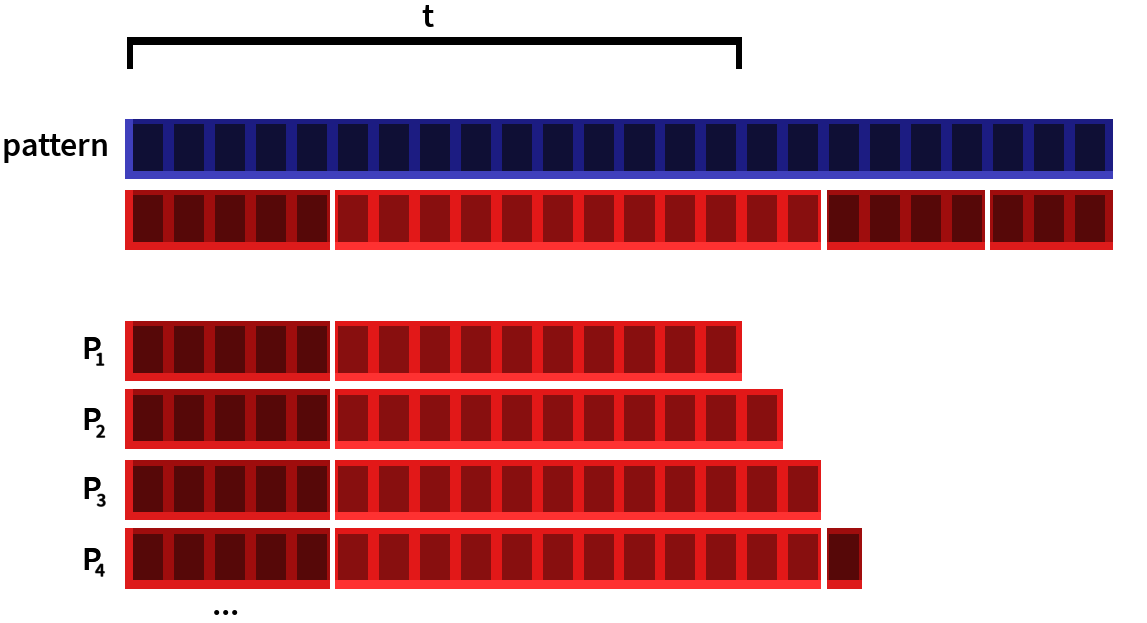
\includegraphics[width=0.7\textwidth]{images/short_block.png}
}
\caption[Short final block in some prefix of a pattern demonstrated]{Prefixes $P_1...P_4$ of some pattern string, where the length of $P_4$ induces a short final block from the pattern's block sequence.}
\label{fig:short_block}
\end{figure}
 
To remedy this problem, \vali{} had a number of ideas which involved passing over the same prefix a number of times, each time offsetting the partitioning divisions on the pattern, and selectively disabling candidate generation whenever these short blocks were predicted to arise. Without dwelling too much on the specifics, this approach was able to cumulatively cover all \glspl{solution} and avoid having to output candidates in cases with extremely short queries. However, it required several passes over the same pattern.





\subsection{\vali{}'s Second Schemes}

\label{schemes:vali2}
Following up their previous paper, \vali{} proposed a new \gls{filtering scheme} to sidestep the problem of short \glspl{block} that plagued their previous algorithm.
 
\begin{fscheme}[Valimaki's Filters]
\textup{For a pattern with N blocks}
\label{valifilters}
\begin{align*}
filters &= \{f_1, f_2\ldots{}, f_{(N-1)}\}\\
f_1 &= [1, 2,\ldots , N]\\
where\phantom{ }X \neq 1 : f_X &= [0, 1, 2,\ldots, X-1]
\end{align*}
\end{fscheme}

\noindent
The new filtering scheme had a new desirable property; To cover all \glspl{solution} for any \gls{pattern} of $K+1$ blocks, the very shortest \gls{filter} (composed of a single block) could be entirely omitted. For the algorithm, this meant that a solution for any prefix of the pattern would be covered even if all searches did not generate \glspl{candidate} until the end of the complete first block. The new algorithm was able to output candidates in just one \gls{text index} \gls{query} per filter. To cover cases that would ordinarily only be found by the missing \gls{query}, the first (largest) \gls{filter} that all prefixes would have in common has its \bfit{pE} 1 larger in all positions than in filtering scheme \ref{karkfilters}; This can be achieved in the search by initializing $\textit{pE} = 1$ instead of 0, giving the branching a head start. As a consequence of the wider search tree, more time is spent in the \gls{search step}. However, the increase in search time is vastly outweighed by the \textit{decrease} in time spent in the \gls{verification step} when using filtering scheme \ref{karkfilters}.






\subsection{Kucherov's Schemes}
\label{schemes:kuch}

In the fashion of \vali{}'s second paper, Kucherov attempted to make an improvement to the earlier algorithm of \vali{}'s first paper by fixing the short first \gls{block} problem. Kucherov offered a new \gls{filtering scheme} that achieved this in a new way.

\begin{fscheme}[Kucherov's Filters]
\textup{For a pattern with N blocks, given a positive integer $S$}
\label{kuchfilters}
\begin{align*}
filters &= \{f_0, f_1\ldots{}, f_{(N+S-1)}\}\\
f_X &= [0, 1, 2,\ldots , X-S]
\end{align*}
\end{fscheme}

Instead of each prefix having $K+1$ partition blocks (for error limit $K$), Kucherov's solution relies on $K+S$ blocks for each prefix, with $S\geq2$. This could be interpreted as guaranteeing $S$ error-free blocks up from just one. This change increases the breadth of search trees, but avoids many \textit{spurious} candidates from being generated, thereby saving time in the \gls{verification step}; The key observation is that the unavoidable \textit{short last block} can now no longer be the \textit{only} block matched for any candidate; Hence, no candidate will be generated with less than one \textit{complete} block's worth of symbols matched.

The correctness of this algorithm can be seen from lemma \ref{lemma0}, a more generalized version of lemma \ref{lemma1}.

\begin{lemma}
\label{lemma0}
If a string containing no more than $K$ symbols $\phi{}$ is partitioned into $K+S$ blocks for $S \geq 0$, at least $S$ blocks must have $0$ $\phi{}$'s.
\end{lemma}

In Kucherov’s canonical example, $S=2$ (where $S=1$ in \vali{}’s first algorithm), but any positive value of $K$ remains correct. With more finely-partitioned prefix patterns, the \gls{filtering scheme} could safely assume that each \gls{solution} would contain more \gls{error}-free blocks, and match more blocks before generating \glspl{candidate}. So far, the assumption of the 0-error blocks occurring as the \textit{first} block in each query only holds because queries are generated to exhaustively guarantee the correctness of the algorithm \textit{using all} queries (essentially branching into a \textit{case distinction} for which each case covers one position for the 0-error block). Creating queries relying on the \textit{specific} position any \textit{subsequent} 0-error blocks in the \gls{block sequence} (for example, the 2nd of two for $S=2$) would require \textit{another} layer of case-distinction, resulting in a number of filters and queries quadratic in the number of blocks, rather than linear. To avoid this, the position of subsequent blocks is not nailed down at all, and \bfit{pE} continues to be incrimented until the last possible moment; In effect, this simply requires that 0-error blocks number 2 to $S$ occur \textit{somewhere} in the block sequence after the first 0-error block. This reasoning is based on lemma \ref{lemma2}.

In addition to guaranteeing more complete blocks matched per candidate, increasing $S$ results in more balanced (albeit increased) work across filters. In a sense, small values of $S$ cause the algorithm to approach the \kark{} algorithm, while large values of $S$ cause it to degenerate towards the filter-free \gls{text index} algorithm from Section \ref{P2text_index}; (The advantage of using blocks at all falls away as blocks get shorter.)
 
In the previous filtering schemes with uniformly-increasing \bfit{pE}, \glspl{filter} of all lengths were prefixes of one another. This is not the case for these Kucherov filters. For searches intended to traverse all prefix lengths (and thus, apply all lengths of \gls{suffix filter}) in tandem, this requires the search path to \textit{fork} at each new block, with some branches accruing an extra \bfit{pE}, and others matching $S-1$ blocks, generating candidates and terminating. Figure \ref{fig:pE_fork} demonstrates this branching search path for $S = 2$. 


\begin{figure}[!htb]
\centering
\makebox[\linewidth][c]{%
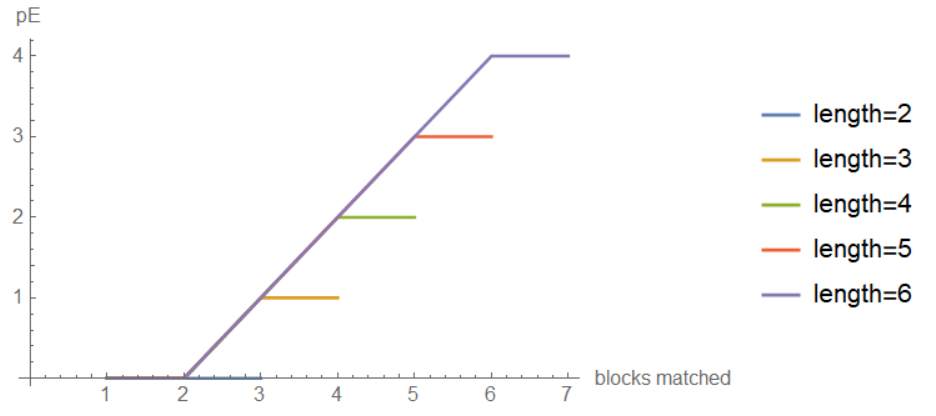
\includegraphics[width=0.8\textwidth]{images/pE.png}
}
\caption[Permitted error variable at various depths in the search tree for per filter length.]{Variable \bfit{pE} `permitted error' at various depths in the search tree (measured per block) for different filter lengths.}
\label{fig:pE_fork}
\end{figure}

Instead of forking the search path, the \gls{candidate condition} can be strengthened to suppress candidate generation for search branches with $\bfit{pE} < S-1$; This achieves the same result of forking the branches, but requires a constant-time check instead of actually forking branches.
